\chapter{Studi Literatur}

Pada bab ini akan mendeskripsikan kajian literatur yang terkait dengan persoalan tugas akhir. Studi literatur ini akan dijadikan dasar dalam melakukan penyelesaian persoalan.

\section{Penggunaan \textit{Spreadsheet}}
Secara harafiah, \textit{spreadsheet} adalah suatu perangkat lunak yang dapat melakukan kalkulasi terhadap angka serta mengorganisir informasi yang ada di dalamnya berdasarkan kolom dan baris \parencite{meriamwebster-spreadsheet}. \textit{Spreadsheet} dapat digunakan untuk melakukan kalkulasi terhadap suatu rumus atau formula yang sulit jika dikalkulasikan dengan cara manual. Selain itu, \textit{spreadsheet} dapat juga digunakan untuk melakukan ramalan terhadap suatu perubahan variabel masukan. Pada perkembangannya, \textit{spreadsheet} memiliki fitur-fitur tambahan seperti visualisasi data dan ekstraksi data penting dari kumpulan data yang ada.

Penelitian tentang penggunaan \textit{spreadsheet} pada bisnis pernah dilakukan sebelumnya pada tahun 2014. Subjek yang diteliti adalah akuntan manajemen \parencite{Bradbard2014}. Pada penelitian tersebut, didapatkan gambaran umum mengenai penggunaan \textit{spreadsheet} secara umum. Menurut hasil penelitian tersebut beberapa fitur yang sering digunakan oleh pengguna \textit{spreadsheet} secara terurut dari yang paling sering digunakan adalah sebagai berikut,

\begin{enumerate}
    \item Menghitung fungsi matematika dasar (tambah, kurang, kali, bagi, dan lainnya)
    \item Mengelola \textit{worksheet} dan \textit{workbook} (menambahkan, menghapus, merubah nama, dan lainnya)
    \item Melakukan perubahan format dasar (menebalkan, memberi garis bawah, format angkat, dan lainnya)
    \item Melakukan pengurutan data, penghitungan subtotal, serta meringkas data
    \item Menggunakan fitur \textit{cell addressing} baik absolut maupun relatif
    \item Penggunaan fungsi kondisi (IF, COUNTIF), fungsi logika (AND, OR), fungsi pencarian (VLOOKUP, HLOOKUP), menautkan \textit{workbook} lain, serta fungsi pembulatan (ROUND, CEILING, FLOOR)
\end{enumerate}

Penggunaan \textit{spreadsheet} sangat bergantung kepada domain bisnis atau organisasi yang menggunakan. Pada bisnis yang berorientasi komersial, \textit{spreadsheet} dapat digunakan sebagai alat bantu perhitungan laba, pengeluaran, investasi, dan pajak. Pada organisasi-organisasi non komersial, \textit{spreadsheet} dapat digunakan sebagai salah satu bentuk basis data yang menangani penyimpanan, pengelolaan, dan pengumpulan data yang mudah dan cepat.

\section{Kesalahan dalam Penggunaan \textit{Spreadsheet}}
Penelitian telah dilakukan oleh Panko \parencite{Panko1998} untuk mengetahui banyaknya kesalahan yang terjadi pada pengembangan \textit{spreadsheet} terutama pada sektor bisnis. Dari penelitian ini, didapatkan bahwa 20\% hingga 40\% \textit{spreadsheet} mengandung kesalahan. Pada kasus tertentu, bahkan ditemukan 90\% \textit{spreadsheet} yang diteliti memiliki kesalahan \parencite{Journal1996}. 

Penelitian yang dilakukan oleh Panko juga menemukan 88\% dari 113 \textit{spreadsheet} yang diaudit melalui 7 lebih studi yang diteliti. Beberapa hasil yang telah di rangkum oleh penelitian tersebut mengunakan \textit{spreadsheet} yang digunakan di dunia nyata dapat dilihat pada Tabel \ref{StudiKesalahan}.
  \begin{longtable}{ | p{3cm} | r | R{2cm} | r | r | r | l | }
    \caption{Studi terhadap Kesalahan pada \textit{Spreadsheet}}
    \label{StudiKesalahan}\\ \hline
    \centering\bfseries{Pembuat} & \bfseries{Tahun} & \centering\bfseries{Jumlah yang Diaudit} & \bfseries{Rata-rata Sel} & \bfseries{Persentase Error} \\ \hline
    \endfirsthead
    \hline
    \centering\bfseries{Pembuat} & \bfseries{Tahun} & \centering\bfseries{Jumlah yang Diaudit} & \bfseries{Rata-rata Sel} & \bfseries{Persentase Error} \\ \hline
    \endhead
    Davies \& Ikin & 1987 & 19 & - & 21\% \\ \hline
    Cragg \& King & 1992 & 20 & 50 - 10000 & 25\% \\ \hline
    Butler & 1992 & 273 & - & 11\% \\ \hline
    Dent & 1994 & Tidak diketahui & - & 30\% \\ \hline
    Hicks & 1995 & 1 & 3856 & 100\% \\ \hline
    Coopers \& Lybrand & 1997 & 23 & 150+ & 91\% \\ \hline
    KPMG & 1998 & 22 & - & 91\% \\ \hline
    Lukasic & 1998 & 2 & 2270 - 7027 & 100\% \\ \hline
    Butler & 2000 & 7 & - & 86\% \\ \hline
    Clermont, Hanin, \& Mittermeier & 2002 & 3 & - & 100\% \\ \hline
    Lawrence and Lee & 2004 & 30 & 2182 & 100\% \\ \hline
    Powell, Lawson, and Baker & 2007 & 25 & - & 64\% \\ \hline
    Powell, Baker \& Lawson & 2007 & 50 & - & 86\% \\ \hline
  \end{longtable}
Dari kumpulan data diatas, dapat dilihat bahwa didalam pembentukan \textit{spreadsheet} pada bidang bisnis, tidak mungkin terlepas dari kesalahan. Dengan tingginya tingkat kesalahan ini, bisnis dapat mengalami kerugian secara material maupun moral yang cukup besar \parencite{EUSPRIGHorrorStories}. Hal ini mengindikasikan bahwa tingginya tingkat kesalahan harus dapat diselesaikan agar tidak terjadi kerugian di dalam penggunaan \textit{spreadsheet} terutama dalam bisnis.

\section{Tipe Kesalahan dalam Penggunaan \textit{Spreadsheet}}
Tingkat fleksibilitas \textit{spreadsheet} yang tinggi memberikan keleluasaan kepada penggunanya untuk melakukan banyak manipulasi dan pengelolaan data. Tingginya fleksibilitas ini dapat berakibat mudahnya \textit{human error} terjadi pada saat penggunaan \textit{spreadsheet} yang menyebabkan terjadinya kesalahan-kesalahan pada data. Tipe-tipe kesalahan pada \textit{spreadsheet} dapat dibagi menjadi dua jenis tipe kesalahan yakni kesalahan kuantitatif, dan kesalahan kualitatif \parencite{Panko1998}. 

    \subsection{Kesalahan Kualitatif}
    Kesalahan kualitatif merupakan kesalahan yang berhubungan dengan kualitas \textit{spreadsheet} tersebut. Beberapa kesalahan yang dapat diklasifikasikan sebagai kesalahan kualitatif adalah \parencite{Powell2009}:

    \begin{enumerate}
        \item Melakukan \textit{hard-code} pada suatu angka di dalam formula
        \item Menggunakan formula yang panjang dalam perhitungan
        \item Susunan data yang tidak direncanakan dengan baik
        \item Tidak adanya dokumentasi mengenai \textit{spreadsheet} yang dibuat
    \end{enumerate}

    Kesalahan ini tidak langsung mengakibatkan nilai hasil keluaran yang salah namun menurunkan kualitas dari \textit{spreadsheet} tersebut \parencite{Rajalingham2001}. Selain itu, kesalahan kualitatif dapat menyebabkan kesalahan kuantitatif terutama pada saat penggunaan fungsi analisis \textit{what-if} pada \textit{spreadsheet} \parencite{Panko1998}.

    \subsection{Kesalahan Kuantitatif}
    Kesalahan ini mengakibatkan \textit{spreadsheet} mengeluarkan hasil dan nilai yang salah didalam operasi perhitungannya. Kesalahan kuantitatif dapat dibagi menjadi tiga tipe kesalahan yakni \parencite{Panko1998}:

    \begin{enumerate}
        \item Kesalahan mekanikal (\textit{mechanical error}) yang biasanya terjadi akibat kesalahan pengetikan angka atau rujukan sel yang salah pada suatu formula
        \item Kesalahan logika (\textit{logical error}) yang terjadi pada pembuatan formula yang salah atau penggunaan fungsi yang tidak tepat
        \item Kesalahan akibat kelalaian pada interpretasi situasi atau spesifikasi yang diberikan sehingga \textit{spreadsheet} yang dihasilkan tidak sesuai dengan domain permasalahan yang ada \parencite{Powell2009} (\textit{ommision error})
    \end{enumerate}

\section{Penanganan Kesalahan pada \textit{Spreadsheet}}
Berdasarkan penelitian yang dilakukan oleh Panko \parencite{Panko1998}, dijabarkan beberapa metode untuk menangani dan mengurangi kesalahan yang sering terjadi. Beberapa metode yang dapat digunakan yakni:

    \begin{enumerate}
        \item Membangun \textit{preliminary design} sebelum pembuatan \textit{spreadsheet} agar terdapat perencanaan yang baik di dalam pembangunan data di dalam \textit{spreadsheet}
        \item Melakukan proteksi terhadap sel yang tidak boleh diubah.
        \item Melakukan pengecekan terhadap semua rumus dan formula yang dimasukan bahkan hingga rumus yang cukup sederhana dengan cara melakukan pengecekan manual.
        \item Membuat dokumentasi untuk \textit{spreadsheet} yang dibuat.
        \item Tidak menekan pembuat \textit{spreadsheet} terhadap kesalahan yang dibuat dengan memberikan hukuman. Kesalahan yang terjadi pada \textit{spreadsheet} umumnya masih berada pada batas normal \textit{human error} sehingga memberikan hukuman akan membuat rasa takut dalam melaporkan kesalahan.
        \item Melakukan inspeksi terhadap formula, rumus, dan kode yang dibuat baik oleh individual maupun secara berkelompok.
    \end{enumerate}

\section{Struktur pada Penyimpanan \textit{Spreadsheet}}
Konsep dasar pada \textit{spreadsheet} modern adalah sebuah aplikasi yang berupa sekumpulan sel terdiri dari baris dan kolom yang disebut \textit{sheet}. Sel ini dapat diisi data berupa data mentah maupun formula. Data mentah biasanya berupa angka, teks, tanggal, dan nilai mata uang. Formula merupakan perintah yang dapat dimengerti komputer untuk menghitung dan memanipulasi data pada sel. Data hasil pengolahan dan masukan pada \textit{spreadsheet} pada dasarnya disimpan dalam bentuk sel yang namanya terdiri dari nama kolom dan nilai baris (Contoh: A1 untuk kolom pertama dan baris pertama). Masing-masing sel tersebut akan menyimpan \textit{properties} dari sel yang dapat berupa \textit{value} yang diisikan, format sel, serta format data yang digunakan. 

Pada masing-masing aplikasi, cara penyimpanannya dapat berbeda satu dengan yang lain walaupun memiliki kemiripan. Bagian ini akan dibahas struktur yang digunakan pada tiga jenis aplikasi yang memiliki tipe yang berbeda; Microsoft Excel 2007 (\textit{Offline Spreadsheet}), Open Office (\textit{Offline and Open Source Spreadsheet}), EtherCalc (\textit{Online and Open Source Spreadsheet}), Google Sheet (\textit{Online Spreadsheet}).

    \subsection{Struktur Penyimpanan pada Microsoft Excel 2007}

    \subsection{Struktur Penyimpanan pada Open Office}

    \subsection{Struktur Penyimpanan pada EtherCalc}

    \subsection{Struktur Penyimpanan pada Google Sheet}

\section{\textit{Data Governance}}


\section{Mekanisme Penyimpanan Data}
Jelasin disini alternatif yang mungkin sebagai penyimpanan data buat hasil dari inputan lewat spreadsheet
Juga jelasin kenapa harus menggunakan basisdata buat penyimpanan
mungkin bisa ditulis dan dijelaskan di data governance???? 
masih bingung buat ngehubunginnnya sih :((((


\subsection{Basis Data Relasional}
Basisdata relasional merupakan sebuah basisdata digital yang berbasiskan pada \textit{paper} yang ditulis oleh E. F. Codd pada tahun 1970. Pada basisdata relasional, model data diatur kedalam bentuk tabel atau relasi yang terdiri dari baris dan kolom, dengan sebuah kunci (\textit{key}) unik untuk setiap barisnya. Sebuah tabel mengambarkan koleksi objek atau relasi yang memiliki kesamaan jenis atau sifat dimana setiap kolomnya dapat mengambarkan suatu objek atau relasi yang biasa disebut sebagai \textit{record} \parencite{codd1970relational, OracleRDB}.

    \subsubsection{Struktur Basis Data Relasional}
    \begin{figure}[htb]
        \centering
        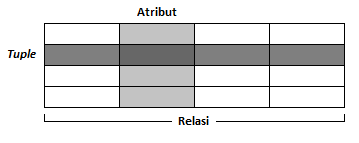
\includegraphics[width=0.6\textwidth]{resources/chapter-2-relational-db.png}
        \caption{Ilustrasi basisdata relasional}
        \label{IlustrasiRDB}
    \end{figure}
    E. F. Codd mendefinisikan basisdata relasional dapat dijelaskan secara sederhana menggunakan representasi tabel atau \textit{array}. Secara terminologi, tabel disebut juga sebagai relasi dan merupakan kumpulan \textit{tuple} yang memiliki atribut yang sama. Atribut direpresentasikan sebagai kolom sedangkan \textit{tuple} direpresentasikan sebagai baris. Gambar \ref{IlustrasiRDB} merupakan ilustrasi dari sebuah tabel pada basisdata relasional.

    Selain terminologi tersebut, tabel atau \textit{array} dapat dikatakan sebuah data yang relasional jika dapat memenuhi beberapa sifat berikut:

    \begin{enumerate}
        \item Setiap baris merepresentasikan sebuah \textit{tuple} sejumlah \textit{n} relasi R
        \item Keterurutan baris tidak perlu diperhatikan (\textit{immaterial})
        \item Setiap baris harus berbeda satu dengan yang lainnya
        \item Keterurutan kolom perlu diperhatikan sesuai dengan domain yang dimodelkan
        \item Setiap kolom diberikan label yang sesuai dengan nama domain yang dimodelkan
    \end{enumerate}

    Sebagai contoh, pada Tabel \ref{ContohTabel} dapat dilihat merupakan contoh sebuah tabel bernama \textit{mahasiswa} dengan 3 derajat relasi yang memiliki atribut NIM, nama, dan jurusan seorang mahasiswa. Setiap baris merupakan kombinasi data yang unik dan tidak berulang.

    \begin{table}[htb]
        \caption{Sebuah relasi pada domain mahasiswa}
        \label{ContohTabel}
        \begin{center}
            \begin{tabular}{ l c c c }
                \hline
                mahasiswa & NIM & nama & jurusan \\
                & 13513042 & Feryandi N. & 135 \\
                & 13613006 & Dani Y. P. & 134 \\
                & 18013024 & Haidar A. D. & 180 \\
                \hline
            \end{tabular}
        \end{center}
    \end{table}

    Konsep lain yang juga dijelaskan oleh Codd adalah adanya \textit{primary key} dan \textit{foreign key}. \textit{Primary key} adalah sebuah nilai unik yang dimiliki oleh sebuah \textit{tuple}, sehingga \textit{tuple} tersebut dapat diidentifikasi secara unik hanya dengan menggunakan nilai tersebut. Pada pemodelan data, relasi satu dengan yang lainnya dapat saling berhubungan hal dapat direpresentasikan menggunakan \textit{foreign key}. Sebuah nilai dapat dikatakan \textit{foreign key} jika nilai tersebut bukanlah merupakan \textit{primary key} pada relasi R, tetapi merupakan \textit{primary key} pada relasi S lainnya \parencite{codd1970relational}. Pada Tabel \ref{ContohTabel}, NIM merupakan \textit{primary key} dari relasi tersebut dan jurusan merupakan \textit{foreign key} yang merujuk ke \textit{primary key} pada tabel relasi lain.

    \subsubsection{\textit{Relational Database Management System (RDBMS)}}

    \subsubsection{Sifat Transaksi pada RDBMS}    

\subsection{Basis Data Non-Relational (NoSQL)}
    
\section{Studi Terkait / Penelitian Terkait}
\blindtext
